\documentclass[12pt,letterpaper,reqno]{article}

% \usepackage{mathtools}
\usepackage{epsfig}
\usepackage{amsmath}
\usepackage{amssymb}
\usepackage{amsthm}
\usepackage{indentfirst}
\usepackage{xspace}
\usepackage{multirow}
\usepackage{hyperref}
\usepackage{xcolor}
\usepackage{verbatim}
\usepackage[letterpaper,margin=1in,headheight=15pt]{geometry}
\usepackage{mathpazo}
\usepackage{tikz-cd}
\usepackage{booktabs}
\usepackage{framed}
\usepackage{float}
\usepackage{thmtools}
\usepackage{dashrule}
\usepackage[missing=]{gitinfo2}
\usepackage{fancyhdr}
\usepackage{enumerate}
\usepackage{graphicx}
\usepackage{mathrsfs}
\usepackage{calligra}
\usepackage[titletoc,title]{appendix}
\usepackage{tikz}
\usetikzlibrary{decorations.markings}
\usetikzlibrary{arrows}

\definecolor{darkblue}{rgb}{0.1,0.1,0.7}
\definecolor{darkred}{rgb}{0.5,0.1,0.1}
\definecolor{darkgreen}{rgb}{0.0,0.42,0.06}
\hypersetup{colorlinks=true,urlcolor=darkred,linkcolor=darkblue,citecolor=darkred}
\definecolor{shadecolor}{rgb}{0.85,0.85,0.85}

% Bibliography formatting
\usepackage[bibstyle=authoryear-comp,labeldate=false,defernumbers=true,maxnames=20,uniquename=init,dashed=false,backend=biber,sorting=none]{biblatex}

\DeclareNameAlias{sortname}{first-last}

\DeclareFieldFormat{url}{\url{#1}}
\DeclareFieldFormat[article]{pages}{#1}
\DeclareFieldFormat[inproceedings]{pages}{\lowercase{pp.}#1}
\DeclareFieldFormat[incollection]{pages}{\lowercase{pp.}#1}
\DeclareFieldFormat[article]{volume}{\textbf{#1}}
\DeclareFieldFormat[article]{number}{(#1)}
\DeclareFieldFormat[article]{title}{\MakeCapital{#1}}
\DeclareFieldFormat[inproceedings]{title}{#1}
\DeclareFieldFormat{shorthandwidth}{#1}

% Don't use "In:" in bibliography. Omit urls from journal articles.
\DeclareBibliographyDriver{article}{%
  \usebibmacro{bibindex}%
  \usebibmacro{begentry}%
  \usebibmacro{author/editor}%
  \setunit{\labelnamepunct}\newblock
  \MakeSentenceCase{\usebibmacro{title}}%
  \newunit
  \printlist{language}%
  \newunit\newblock
  \usebibmacro{byauthor}%
  \newunit\newblock
  \usebibmacro{byeditor+others}%
  \newunit\newblock
  \printfield{version}%
  \newunit\newblock
%  \usebibmacro{in:}%
  \usebibmacro{journal+issuetitle}%
  \newunit\newblock
  \printfield{note}%
  \setunit{\bibpagespunct}%
  \printfield{pages}
  \newunit\newblock
  \usebibmacro{eprint}
  \newunit\newblock
  \printfield{addendum}%
  \newunit\newblock
  \usebibmacro{pageref}%
  \usebibmacro{finentry}}

% Remove dot between volume and number in journal articles.
\renewbibmacro*{journal+issuetitle}{%
  \usebibmacro{journal}%
  \setunit*{\addspace}%
  \iffieldundef{series}
    {}
    {\newunit
     \printfield{series}%
     \setunit{\addspace}}%
  \printfield{volume}%
%  \setunit*{\adddot}%
  \printfield{number}%
  \setunit{\addcomma\space}%
  \printfield{eid}%
  \setunit{\addspace}%
  \usebibmacro{issue+date}%
  \newunit\newblock
  \usebibmacro{issue}%
  \newunit}


% Bibliography categories
\def\makebibcategory#1#2{\DeclareBibliographyCategory{#1}\defbibheading{#1}{\section*{#2}}}
\makebibcategory{books}{Books}
\makebibcategory{papers}{Refereed research papers}
\makebibcategory{chapters}{Book chapters}
\makebibcategory{conferences}{Papers in conference proceedings}
\makebibcategory{techreports}{Unpublished working papers}
\makebibcategory{bookreviews}{Book reviews}
\makebibcategory{editorials}{Editorials}
\makebibcategory{phd}{PhD thesis}
\makebibcategory{subpapers}{Submitted papers}
\makebibcategory{curpapers}{Current projects}

\setlength{\bibitemsep}{2.65pt}
\setlength{\bibhang}{.8cm}
\renewcommand{\bibfont}{\small}

\renewcommand*{\bibitem}{\addtocounter{papers}{1}\item \mbox{}\hskip-0.85cm\hbox to 0.85cm{\hfill\arabic{papers}.~~}}
\defbibenvironment{bibliography}
{\list{}
  {\setlength{\leftmargin}{\bibhang}%
   \setlength{\itemsep}{\bibitemsep}%
   \setlength{\parsep}{\bibparsep}}}
{\endlist}
{\bibitem}

\newenvironment{publications}{\section{\LARGE Publications}\label{papersstart}\vspace*{0.2cm}\small
\titlespacing{\section}{0pt}{1.5ex}{1ex}\itemsep=0.00cm
}{\label{papersend}\addtocounter{sumpapers}{-1}\refstepcounter{sumpapers}\label{sumpapers}}

\def\printbib#1{\printbibliography[category=#1,heading=#1]\lastref{sumpapers}}

% Counters for keeping track of papers
\newcounter{papers}\setcounter{papers}{0}
\newcounter{sumpapers}\setcounter{sumpapers}{0}
\def\lastref#1{\addtocounter{#1}{\value{papers}}\setcounter{papers}{0}}

% theorem environments
\declaretheoremstyle[spaceabove=0.25cm,spacebelow=0.25cm,notefont=\normalfont\bfseries, notebraces={(}{)}]{theorem}
\declaretheoremstyle[spaceabove=0.25cm,spacebelow=0.25cm,bodyfont=\normalfont,notefont=\normalfont\bfseries, notebraces={(}{)}]{noital}
\declaretheoremstyle[spaceabove=0.25cm,spacebelow=0.25cm,bodyfont=\normalfont\color{darkgreen},notefont=\normalfont\bfseries, notebraces={(}{)}]{green}
\declaretheoremstyle[spaceabove=0.25cm,spacebelow=0.25cm,bodyfont=\normalfont,notefont=\normalfont\bfseries,qed=$\qedsymbol$,notebraces={(}{)}]{proofstyle}

\declaretheorem[name=Theorem,numberwithin=section,style=theorem]{thm}
\declaretheorem[name=Proposition,sibling=thm,style=theorem]{prop}
\declaretheorem[name=Corollary,sibling=thm,style=theorem]{cor}
\declaretheorem[name=Lemma,sibling=thm,style=theorem]{lem}
\declaretheorem[name=Definition,sibling=thm,style=noital]{defn}
\declaretheorem[name=Example,sibling=thm,style=noital]{example}
\declaretheorem[name=Exercise,numberwithin=section,style=green]{exercise}
\declaretheorem[name=Proof,style=proofstyle,numbered=no]{pf}

\numberwithin{equation}{section}


% macros for convenience
\newcommand{\tops}{\texorpdfstring}

\newcommand{\nid}{\noindent}

\newcommand{\fa}{{\mathfrak a}}
\newcommand{\fp}{{\mathfrak p}}
\newcommand{\fk}{{\mathfrak k}}
\newcommand{\fg}{{\mathfrak g}}
\newcommand{\fh}{{\mathfrak h}}
\newcommand{\fn}{{\mathfrak n}}
\newcommand{\fq}{{\mathfrak q}}
\newcommand{\fm}{{\mathfrak m}}
\newcommand{\fr}{{\mathfrak r}}
\newcommand{\fu}{{\mathfrak u}}
\newcommand{\fG}{{\mathfrak G}}

\newcommand{\cC}{\ensuremath{\mathcal C}}
\newcommand{\cG}{\ensuremath{\mathcal G}}
\newcommand{\cB}{\ensuremath{\mathcal B}}
\newcommand{\cL}{\ensuremath{\mathcal L}}
\newcommand{\cS}{\ensuremath{\mathcal S}}
\newcommand{\cF}{\ensuremath{\mathcal F}}
\newcommand{\cK}{\ensuremath{\mathcal K}}
\newcommand{\cZ}{\ensuremath{\mathcal Z}}
\newcommand{\cM}{\ensuremath{\mathcal M}}
\newcommand{\cN}{\ensuremath{\mathcal N}}
\newcommand{\cO}{\ensuremath{\mathcal O}}
\newcommand{\cH}{\ensuremath{\mathcal H}}
\newcommand{\cX}{\ensuremath{\mathcal X}}
\newcommand{\cY}{\ensuremath{\mathcal Y}}
\newcommand{\cA}{\ensuremath{\mathcal A}}
\newcommand{\cI}{\ensuremath{\mathcal I}}

\newcommand{\R}{\ensuremath{\mathbb R}}
\newcommand{\C}{\ensuremath{\mathbb C}}
\newcommand{\PP}{\ensuremath{\mathbb P}}
\newcommand{\Z}{\ensuremath{\mathbb Z}}
\newcommand{\Q}{\ensuremath{\mathbb Q}}
\newcommand{\A}{\ensuremath{\mathbb A}}
\newcommand{\bbH}{\ensuremath{\mathbb H}}
\newcommand{\bbI}{\ensuremath{\mathbb I}}
\newcommand{\bS}{\ensuremath{\mathbb S}}

\newcommand{\half}{\ensuremath{\frac{1}{2}}}
\newcommand{\qtr}{\ensuremath{\frac{1}{4}}}
\newcommand{\bq}{{\mathbf q}}
\newcommand{\N}{{\mathcal N}}
\newcommand{\F}{{\mathcal F}}
\newcommand{\HH}{{\mathcal H}}
\newcommand{\LL}{{\mathcal L}}
\newcommand{\RR}{{\mathcal R}}
\newcommand{\V}{{\mathcal V}}
\newcommand{\dirac}{\!\!\not\!\partial}
\newcommand{\Dirac}{\!\!\not\!\!D}
\newcommand{\cE}{{\mathcal E}}
\newcommand{\vs}{\not\!v}
\newcommand{\kahler}{K\"ahler\xspace}
\newcommand{\kq}{/\!\!/}
\newcommand{\kql}[1]{/\!\!/\!\!_#1\,}
\newcommand{\hk}{hyperk\"ahler\xspace}
\newcommand{\Hk}{Hyperk\"ahler\xspace}
\newcommand{\hkq}{/\!\!/\!\!/\!\!/}
\newcommand{\hkql}[1]{/\!\!/\!\!/\!\!/\!\!_#1\,}
\newcommand{\del}{\ensuremath{\partial}}
\newcommand{\delbar}{\ensuremath{\overline{\partial}}}
\newcommand{\I}{{\mathrm i}}
\newcommand{\J}{{\mathrm j}}
\newcommand{\K}{{\mathrm k}}
\newcommand{\e}{{\mathrm e}}
\newcommand\bid{{\mathbf 1}}
\newcommand{\de}{\mathrm{d}}
\newcommand{\ab}{\mathrm{ab}}
\newcommand{\vol}{\mathrm{vol}}
\renewcommand{\sf}{\mathrm{sf}}
\newcommand{\inst}{\mathrm{inst}}
\newcommand{\eff}{\mathrm{eff}}
\newcommand{\dR}{\mathrm{dR}}
\newcommand{\closed}{\mathrm{closed}}
\newcommand{\exact}{\mathrm{exact}}

\newcommand{\abs}[1]{\lvert#1\rvert}
\newcommand{\norm}[1]{\lVert#1\rVert}
\newcommand{\IP}[1]{\langle#1\rangle}
\newcommand{\DIP}[1]{\langle\!\langle#1\rangle\!\rangle}
\newcommand{\dwrt}[1]{\frac{\partial}{\partial#1}}
\newcommand{\eps}{\epsilon}
\newcommand{\simarrow}{\xrightarrow\sim}

\newcommand{\mmaref}[1]{}

\newcommand{\ti}[1]{\textit{#1}}
\newcommand{\tb}[1]{\textbf{#1}}
\newcommand{\lo}{\text{\calligra o}\,}
\newcommand{\dd}{\ensuremath{\mathscr{D}}}
\newcommand{\sgn}{\text{sgn}}


\DeclareMathOperator{\ad}{ad}
\DeclareMathOperator{\im}{Im}
\DeclareMathOperator{\re}{Re}
\DeclareMathOperator{\Tr}{Tr}
\DeclareMathOperator{\End}{End}
\DeclareMathOperator{\Hom}{Hom}
\DeclareMathOperator{\Aut}{Aut}
\DeclareMathOperator{\Sym}{Sym}
\DeclareMathOperator{\Lie}{Lie}
\DeclareMathOperator{\diag}{diag}
\DeclareMathOperator{\Bun}{Bun}
\DeclareMathOperator{\Vect}{Vect}
\DeclareMathOperator{\Span}{Span}
\DeclareMathOperator{\grad}{grad}
\DeclareMathOperator{\rank}{rank}
\DeclareMathOperator{\ind}{ind}
\DeclareMathOperator{\coker}{coker}
\DeclareMathOperator{\Jac}{Jac}
\DeclareMathOperator{\Hol}{Hol}
\DeclareMathOperator{\gr}{gr}

\newcommand{\insfig}[2]{

\medskip
\noindent
\begin{minipage}{\linewidth}

\makebox[\linewidth]{\includegraphics[keepaspectratio=true,scale=#2]{figures/#1-crop.pdf}}

\end{minipage}
\medskip

}


% \newcommand{\insfig}[2]{\begin{figure}[htbp] \centering \includegraphics[scale=#2]{figures/#1-crop.pdf} \label{fig:#1} \end{figure}}
% syntax: \insfig{name}{0.5}{caption}

\newcommand{\fixme}[1]{{\color{orange}{[#1]}}}
\newcommand{\currentposition}{{\color{blue} \noindent\makebox[\linewidth]{\hdashrule{\paperwidth}{1pt}{3mm}}}}

% \mathtoolsset{showonlyrefs}

\bibliography{mvc}

\begin{document}
\pagestyle{fancy}
\lhead{{\tiny \color{gray} \tt \gitAuthorIsoDate}}
\chead{\tiny \ti{Linear Algebra, GSMST 2018-2019}}
\rhead{{\tiny \color{gray} \tt \gitAbbrevHash}}
\renewcommand{\headrulewidth}{0.5pt}


\begin{center}
\tb{Multivariable Calculus \\
Semester 1: Linear Algebra} \\
Anderson Trimm \\
Gwinnett School of Mathematics, Science and Technology \\
\end{center}

{These are the notes for the Fall Semester 2019
of Multivariable Calculus at GSMST, which covers linear algebra. They will updated frequently throughout the semester. The latest PDF can always be accessed
at \small \url{https://github.com/atrimm/mvc/blob/master/Course%20Notes/linear_algebra_2019.pdf}.} Please email me with comments and corrections, or send them to me directly as pull requests to the source repository hosted at \small \url{https://github.com/atrimm/mvc}.

\tableofcontents
\renewcommand{\listtheoremname}{Quick reference}
\listoftheorems[onlynamed]

\newpage

%\setcounter{page}{1}
\section{Vectors and geometry}
\subsection{Physical motivation}
The earliest notion of a \emph{vector} comes from physics. In nature, we encounter certain physical quantities which cannot be uniquely specified by a number alone, but also depend on a direction in space. 

\begin{example}\label{ex:disp}
If the distance from town $A$ to town $B$ is 400 miles and we leave $A$ and travel at 50 miles per hour, then we will arrive at $B$ in 8 hours, but only if we travel in the direction from $A$ to $B$! Thus, displacement (400 mi, from $A$ to $B$) and velocity (50 mi/hr, from $A$ to $B$) are two examples of such physical quantities.
\end{example}
To distinguish physical quantities which depend on a numerical value alone from those which also depend on a direction, we make the following definitions. 
\begin{defn}[Vectors and scalars]
\begin{enumerate}[(a)] \hspace{10cm}
	\item A \emph{scalar} is a physical quantity which is uniquely specified by a numerical value alone.
	\item A \emph{vector} is a physical quantity which is uniquely specified by a numerical value, called its \emph{magnitude}, and a direction.
\end{enumerate}
\end{defn}

\begin{exercise}
Classify each of the following quantities are vector or scalar:
\begin{enumerate}[(a)]
	\item Force
	\item Temperature
	\item Mass
	\item Volume
	\item Acceleration
	\item Electric Charge
	\item Density
\end{enumerate}	
\end{exercise}

In the following sections, we will develop a mathematical model of vector and scalar quantities capable of modeling physical phenomena. As we will see, this model will have applications beyond physics as well.

\subsection{Mathematical model}
\subsubsection{Scalars}\label{sec:scalars}
While electric charges are observed in nature to take only integer values, other scalar quantities, such as mass and temperature, are found to take any \emph{real} value. Thus, in our model a scalar is simply a real number. We denote the set of all real numbers by $\mathbb{R}$. We will denote a scalar by a lower case latin letter, such as $x$.

\subsubsection{Vectors}
A vector quantity is uniquely specified by two pieces of information: a magnitude (which is a nonnegative real number) and a direction in three-dimensional space. We can therefore represent a vector geometrically as an \emph{arrow} (directed line segment) in space.  The arrow points in the direction specifying the vector while the length of the arrow represents the magnitude of the vector. For example, a force of 25 N directed at an angle of $45^\circ$ with respect to the positive $x$-axis is represented by the arrow \fixme{Insert graphic.} We will denote a vector by a boldface latin letter (either upper or lowercase), such as $\mathbf{x}$. When writing by hand, a more common notation is $\vec{x}$.

\subsubsection{Equality of vectors}
We will now discuss the notion of equivalence of two vectors. Recall first the equivalence of plane figures, say triangles. We consider two distinct triangles. Since the data defining a triangle are the side lengths and interior angle measures, any two triangles related by a transformation which leaves these unchanged represents an equivalent triangle; the only difference between them is the location in the plane. As you learned in basic algebra, any transformation of the plane which preserves lengths and angles can be written as a finite sequence of reflections, translations, and rotations and any two triangles related by such a transformation are said to be \emph{congruent}. 

Since the defining data of a vector is the magnitude and direction, we will agree that

\begin{defn}[Equality of vectors]
Two vectors are equal if they have the same magnitude and direction.	
\end{defn}
That is, two vectors are equal if they are represented by parallel line segments which have the same length and orientation. 

\begin{center}
	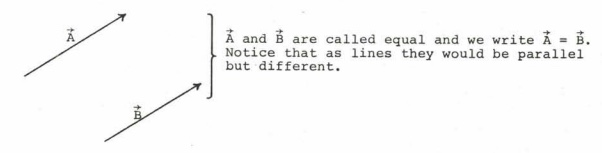
\includegraphics[scale=0.5]{figures_mvc/equal_vectors_new}
\end{center}
If two vectors $\mathbf{x}$ and $\mathbf{y}$ are equal, we will denote this by $\mathbf{x}=\mathbf{y}$.

It is important to note that we have defined equality of vectors so that \emph{location} in space does \emph{not} matter. As line segments, the two parallel arrows are congruent, \footnote{Since they have the same length; the fact that they are parallel or have the same orientation does not matter.} but still considered distinct due to their difference in location, but as \emph{vectors} they are regarded as exactly the same vector.

\subsection{Vector arithmetic}
We will now define operations involving vectors, whose motivation will come from physics. \footnote{In defining operations on the set of vectors, it is important that we have explicitly stated when two vectors are to be regarded being equal, as this will be needed to ensure that our definitions make sense. For instance, consider the definition of addition of rational numbers:
\begin{align}\label{eq:sum_good}
	\frac{m}{n}+\frac{p}{q}=\frac{mq+np}{nq}.
\end{align}
Suppose instead we try to define addition by 
\begin{align}\label{eq:sum_bad}
	\frac{m}{n}+\frac{p}{q}=\frac{m+p}{n+q}.
\end{align}
With this definition, we have, for example,
	$\frac{1}{2}+\frac{1}{3}=\frac{1+1}{2+3}=\frac{2}{5}$.
Now, in both these definitions, the formula for the sum has a \emph{massive} built-in ambiguity: the symbol ``$\frac{1}{2}$" is just one representative of the infinite set $\{\frac{1}{2}, \frac{2}{4}, \frac{3}{6},\dots\}$. Therefore the sum
	$\frac{1}{2}+\frac{1}{3}$
should be equivalent to 
	$\frac{2}{4}+\frac{3}{9}$.
However, with definition \eqref{eq:sum_bad}, we have
$\frac{1}{2}+\frac{1}{3}=\frac{2}{5}$
while
$\frac{2}{4}+\frac{3}{9}=\frac{5}{13}$
and $\frac{2}{5} \neq \frac{5}{13}$. Thus definition \eqref{eq:sum_bad} makes \emph{absolutely no sense}.

On the other hand, using the proper definition \eqref{eq:sum_good}, we have
	$\frac{1}{2}+\frac{1}{3}=\frac{5}{6}$
while
$\frac{2}{4}+\frac{3}{9}=\frac{30}{36}$ 
and indeed $\frac{5}{6}=\frac{30}{36}$ as rational numbers.

To see what went wrong for \eqref{eq:sum_bad}, note that the operation in both \eqref{eq:sum_bad} and \eqref{eq:sum_good} required \emph{choosing} one of the elements of the sets $\{\frac{1}{2},\frac{2}{4},\dots\}$ and $\{\frac{1}{3},\frac{3}{9},\dots\}$ and applying the formula on the right hand side. For the definition to make sense, the result of the operation must be \emph{independent} of this choice. We describe this issue by saying that we have to verify that our proposed operation is \emph{well-defined}.}

\subsubsection{Vector addition}
The most basic operation one can define on a set is a \emph{binary operation}, which is a rule for combining any two elements in the set to produce a third element in the set. \footnote{More formally, we write this as a map $V \times V \to V$, where $V \times V=\{(v,w) \mid v,w \in V\}$ denotes the set of all ordered pairs of elements of $V$, called the \emph{Cartesian product} of $V$ with itself.} There is a natural binary operation on the set of vectors, which is suggested by the \emph{force table} experiment in mechanics.

\begin{center}
	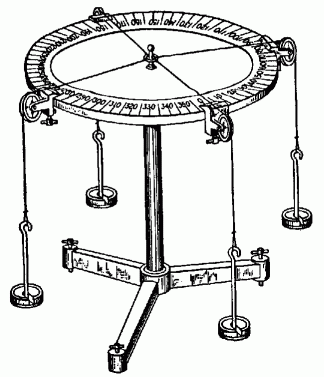
\includegraphics[scale=0.5]{figures_mvc/force_table_experiment_2}
\end{center}

In a force table experiment, strings are tied to a metal ring which is positioned at the center of the table. The strings are then suspended over pulleys which are fixed at known angles, and known masses hung from the ends of the strings. The pull of gravity on a given mass creates tension in the string which pulls on the ring. 

In an experiment in which \emph{two} strings are tied to the ring, the tension in each string gives rise to two forces pulling on the washer in different directions. However, the washer ultimately accelerates in a single direction, which is the direction of the \emph{net} (or \emph{total}) force acting on the ring. The rule for combining the two tension force vectors to produce the net force vector is exactly the binary operation we seek to define. 

To determine the net force, a third string is connected to the ring with mass and pulley position chosen so that the ring is in \emph{static equilibrium} (i.e., it does not move at all under the influence of these three forces). This vector is called the \emph{equilibrant} vector. By Newton's third law, the net force vector (also called the \emph{resultant} vector) is then the \emph{opposite} of the equilibrant vector, that is, it has the same magnitude and is directed along the same line, but with the opposite orientation.

\begin{center}
	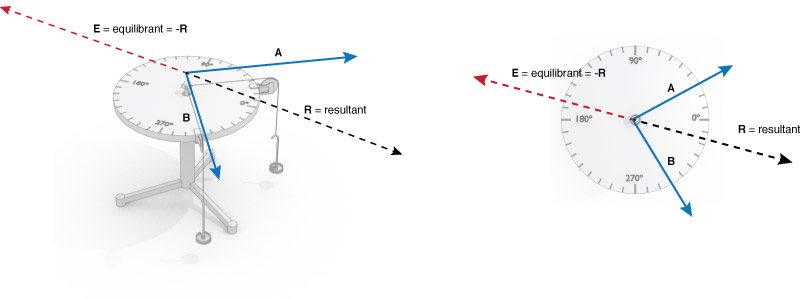
\includegraphics[scale=0.5]{figures_mvc/force-table-equi-res}
\end{center}

 We therefore define the \emph{sum} of two vectors as follows:
 
 \begin{defn}[Vector addition]
 	The \ti{sum} ${\bf v}+{\bf w}$ of two vectors ${\bf v}$ and ${\bf w}$ is the resultant vector of ${\bf v}$ and ${\bf w}$.
 \end{defn}
Note that when the two tension forces are along the \emph{same} direction (e.g., just add another mass on the same string), the resultant vector points in this same direction and has magnitude given by the sum of the magnitudes of the two tension vectors, and hence the addition of ${\bf v}$ and ${\bf w}$ reduces to addition of ordinary numbers in this special case. This is why we have decided to call this binary operation \emph{addition} and to continue to denote it by $+$; it can therefore be thought of as a \emph{generalization} of the ordinary addition of scalars. 
 
In terms of our geometric representation of vectors, the magnitude and direction of ${\bf v}+{\bf w}$ is determined as follows: Since the location of a vector is of no consequence (by our definition of equality of vectors), we may position the two vectors so that their initial points coincide. Then ${\bf v}$ and ${\bf w}$ form adjacent sides of a parallelogram, and the vector ${\bf v}+{\bf w}$ is the diagonal of the parallelogram, directed from the common initial point of ${\bf v}$ and ${\bf w}$ to the opposite vertex of the parallelogram, as shown below.	
\begin{center}
	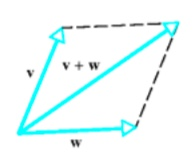
\includegraphics[scale=0.5]{figures_mvc/parallelogram_rule}
\end{center}
This is called the \ti{parallelogram rule} for vector addition. Since the opposite sides of a parallelogram are congruent and parallel, we can equivalently view ${\bf v}+{\bf w}$ as the result of positioning the initial point of ${\bf w}$ at the terminal point of ${\bf v}$ and drawing the arrow connecting the initial point of ${\bf v}$ to the terminal point of ${\bf w}$.

\begin{center}
	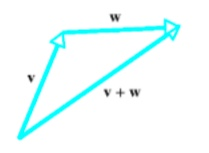
\includegraphics[scale=0.5]{figures_mvc/tip_to_tail}
\end{center}
This is called the \ti{triangle rule} or \ti{``tip to tail" rule} for vector addition. These two points of view are related by \ti{parallel translation}. To go from the first point of view to the second, we translate the initial point of ${\bf w}$ along ${\bf v}$, keeping ${\bf w}$ parallel to its original direction at all times. Accordingly, ${\bf v}+{\bf w}$ is also called the \ti{translation of ${\bf w}$ by ${\bf v}$}.
\begin{center}
	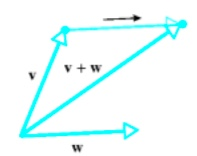
\includegraphics[scale=0.5]{figures_mvc/translation_of_v_by_w}
\end{center}

\begin{example}
There is another physical interpretation of this addition rule which agrees with our intuition. Suppose a person walks 10 steps in a north-easterly direction, and then turns and walks another 5 steps to the east. The vector $\mathbf{v}$ then represents his \emph{displacement} from his initial position, with the length of $\mathbf{v}$ being his distance from where he started, and the direction of $\mathbf{v}$ pointing in the direction in which he moved. Similarly, the vector $\mathbf{w}$ represents his displacement from his position after he traveled along the vector $\mathbf{v}$. Their sum, added according to the tip to tail rule, is his \emph{total} displacement from his initial position.	
\end{example}

Let us now use this geometric picture to determine the properties of vector addition. Recall that the addition operation defined on the set of real numbers satisfies the following properties: \footnote{Any set $G$ on which there is a binary operation $*$ which satisfies the first three of these properties is said to form a \emph{group} under $*$. One also says that $(G,*)$ is a group, or just that $G$ is a group if $*$ is understood. If the fourth property (commutativity) also holds, $G$ is said to form a \emph{commutative} (or \emph{abelian}) under $*$.}
\begin{enumerate}[(i)]
	\item Associativity: $(x+y)+z=x+(y+z)$ for all $x,y,z \in \mathbb{R}$.
	\item Existence of an additive identity: $\mathbb{R}$ contains an element 0 such that $0+x=x$ for every $x \in \mathbb{R}$.
	\item Existence of additive inverses: For every $x \in \mathbb{R}$, there exists and element $y \in \mathbb{R}$ such that $x+y=0$.
	\item Commutativity: $x+y=y+x$ for all $x,y \in \mathbb{R}$.
\end{enumerate}
We now consider each of these in turn. We consider commutativity first, since it is the simplest to analyze.

\begin{prop}[Vector addition is commutative]
	Vector addition is commutative. That is, 
	\begin{align*}
		{\bf v}+{\bf w}={\bf w}+{\bf v}
	\end{align*}
	for any two vectors ${\bf v}$ and ${\bf w}$, since each of these is the diagonal of the parallelogram whose edges are formed by $\mathbf{v}$ and $\mathbf{w}$.
\end{prop}

\begin{pf}
	We see from the two diagrams below that the translation of ${\bf w}$ by ${\bf v}$ is the same vector as the translation of ${\bf v}$ by ${\bf w}$.
\begin{center}
	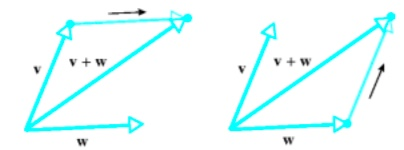
\includegraphics[scale=0.5]{figures_mvc/equivalence_of_vector_addition}
\end{center}

\end{pf}

\begin{prop}[Vector addition is associative]
	Vector addition is associative. That is, for any three vectors ${\bf u}, {\bf v},$ and ${\bf w}$, we have
	\begin{align*}
		{\bf u}+({\bf v}+{\bf w})=({\bf u}+{\bf v})+{\bf w}
	\end{align*}
We therefore denote both expressions by ${\bf u}+{\bf v}+{\bf w}$. 
\end{prop}

\begin{pf}
One can construct ${\bf u}+{\bf v}+{\bf w}$ by placing the vectors ``tip to tail" in succession and then drawing the vector from the initial point of ${\bf u}$ to the terminal point of ${\bf w}$. If the three vectors lie in the same plane, one can verify associativity from the diagram below.
\end{pf}

\begin{center}
	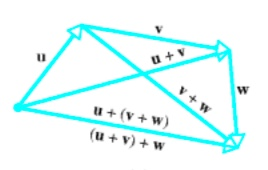
\includegraphics[scale=0.5]{figures_mvc/associativity_of_vector_addition}
\end{center}

If the three vectors do not all lie in the same plane, then when placed at the same initial point the vectors ${\bf u}, {\bf v},$ and ${\bf w}$ from adjacent edges of a \emph{parallelepiped}. \footnote{A parallelepiped is a polygon whose faces are parallelograms, with each pair of opposite sides parallel.} Translating these vectors and adding tip to tail, we see that ${\bf u}+{\bf v}+{\bf w}$ is the diagonal of this parallelepiped.

\begin{center}
	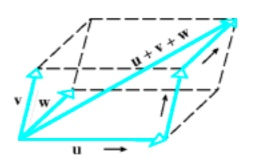
\includegraphics[scale=0.5]{figures_mvc/volume_of_parallelepiped_vectors}
\end{center}

\begin{cor}
The sum ${\bf v}_1+{\bf v}_2+\cdots + {\bf v}_k$ is independent of how the expression is bracketed.	
\end{cor}

\begin{pf}
We postpone the proof until we discuss vectors in coordinates in \fixme{Insert section reference here.}, as the geometry is very complicated and difficult to analyze.	
\end{pf}

Let us now check whether there is a vector which plays the role of an additive identity. That is, given any vector ${\bf b}$, is there a vector ${\bf 0}$ such that ${\bf b}+{\bf 0}={\bf b}$? Let us suppose there is such a vector ${\bf 0}$ and denote its magnitude by $r$. Let us now add ${\bf 0}$ to ${\bf b}$ by the tip-to-tail method. Since ${\bf 0}$ has magnitude $r$, ${\bf b}+{\bf 0}$ must lie on a circle of radius $r$ centered on the tip of ${\bf b}$. However, the condition ${\bf b}+{\bf 0}={\bf b}$ means that ${\bf b}+{\bf 0}$ must have the same magnitude and direction as ${\bf b}$, and there is no point on the circle for which this is true. This shows that there is no such vector ${\bf 0}$ with nonzero length. 
\begin{center}
	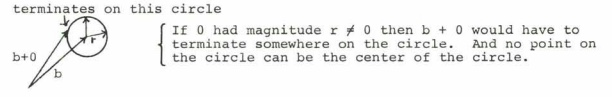
\includegraphics[scale=0.5]{figures_mvc/b_plus_zero_circle}
\end{center}

A vector of length zero, does not have a defined direction. Thus, there is a unique vector which acts as an additive identity with respect to vector addition.

\begin{defn}[The zero vector]
	The zero vector, which we denote by ${\bf 0}$, is the unique vector of magnitude zero.
\end{defn}

Finally, we want to investigate whether every vector has an additive inverse. That is, we want to determine if, when given any vector ${\bf a}$, we can find another vector ${\bf b}$ such that ${\bf a}+{\bf b}={\bf 0}$. Since the zero vector has zero length and since we add vectors from ``tip to tail", it follows that if ${\bf a}+{\bf b}={\bf 0}$, then the tail of ${\bf a}$ and the tip of ${\bf b}$ must coincide. Thus, any vector $\mathbf{a}$ has a \emph{unique} inverse, which we denote by $-\mathbf{a}$.   
\begin{center}
	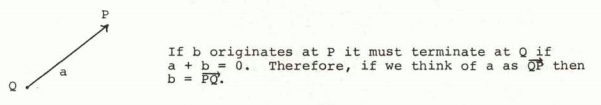
\includegraphics[scale=0.5]{figures_mvc/a_plus_b_equals_zero}
\end{center} 
\begin{defn}[Inverse of a vector]
The additive inverse of a vector ${\bf a}$ is the unique vector $-\mathfrak{a}$, which has the same magnitude as $\mathbf{a}$ and opposite orientation.
\end{defn}
In analogy with the equation $x+(-x)=0$ for real numbers, we denote the additive inverse of ${\bf a}$ by $-{\bf a}$, so that ${\bf a}+(-{\bf a})={\bf 0}$ for any vector ${\bf a}$. We may again agree, as in the case of numerical addition, to abbreviate ${\bf a}+(-{\bf b})$ as ${\bf a}-{\bf b}$, which allows us to define vector subtraction:

\begin{defn}[Vector subtraction]\label{def:vector_subtraction}
	The difference ${\bf a}-{\bf b}$ of two vectors ${\bf a}$ and ${\bf b}$ is the sum
	\begin{align*}
		{\bf a}-{\bf b}={\bf a}+(-{\bf b}).
	\end{align*}
\end{defn}
From this definition, we may view vector subtraction geometrically as follows: To form ${\bf a}-{\bf b}$,
\begin{enumerate}[(1)]
	\item Obtain $(-{\bf b})$ from ${\bf b}$ by reversing the direction of ${\bf b}$.
	\item Add ${\bf a}$ and $(-{\bf b})$ in the usual way, by placing the tail of $(-{\bf b})$ at the tip of ${\bf a}$. \footnote{Like numerical subtraction, vector subtraction is \ti{not} commutative, so the order matters here.}
\end{enumerate}

\begin{center}
	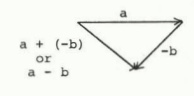
\includegraphics[scale=0.5]{figures_mvc/a_minus_b}
\end{center}

\begin{exercise}
Consider adding vectors ${\bf a}$ and ${\bf b}$ tail-to-tail, as shown below
	\begin{center}
		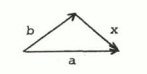
\includegraphics[scale=0.5]{figures_mvc/b_plus_x_equals_a}
	\end{center}
	Show that ${\bf x}={\bf a}-{\bf b}$. This gives another view of vector subtraction which is very useful computationally.
\end{exercise}

{\color{red} \flushleft {\bf Solution:}
We see from the tip-to-tail rule, that ${\bf b}+{\bf x}={\bf a}$. Adding $(-{\bf b})$ to both sides of this equation and using associativity gives ${\bf x}={\bf a}-{\bf b}$.}

The previous exercise shows that, if ${\bf a}$ and ${\bf b}$ are any two vectors and we wish to find ${\bf a}-{\bf b}$, we place the two vectors tail-to-tail and ${\bf a}-{\bf b}$ is then the vector which extends from the tip of ${\bf b}$ to the tip of ${\bf a}$.

We have just shown that our definition of vector addition satisfies the same properties as numerical addition. That is, the additive structures are exactly the same for vectors as for numbers. \footnote{To state this more formally, they both form an abelian group.} Therefore, any results that hold for numbers also hold for vectors, for exactly the same reasons. For example,

\begin{thm}[Cancellation law]
	If ${\bf a}, {\bf b},$ and ${\bf c}$ are vectors such that ${\bf a}+{\bf b}={\bf a}+{\bf c}$, then ${\bf b}={\bf c}$. 
\end{thm}

\begin{pf}
The proof for real numbers is as follows: let $x,y,z$ be real numbers such that 
\begin{align*}
	x+y=x+z
\end{align*}
Adding $-x$ to both sides of this equation, we have
\begin{align*}
	-x+(x+y)&=-x+(x+z) \\
	(-x+x)+y&=(-x+x)+z \text{ (since $+$ is associative)} \\
	0+y&=0+z \text{ (since $-x$ is the inverse of $x$)} \\
	y&=z \text{ (since $0$ is the additive identity)}
\end{align*}
Since addition of vectors obeys exactly the same properties as addition of real numbers, this same proof holds for vectors simply by drawing arrows over $x,y$ and $z$!
\end{pf}

\subsubsection{Scalar multiplication}
In physics, we observe that an unbalanced force on a body causes an acceleration in the direction of the force. It is also observed that the magnitude of acceleration of different bodies, when subjected to the same force, varies according to their mass. These observations are formalized in Newton's second law of motion
\begin{equation}
	{\bf F}=m{\bf a}.
\end{equation}
On the right side of this equation, we see a new operation: the product of a scalar and a vector. 

\begin{defn}[Scalar multiplication]
Let $\mathbf{v}$ be a vector and $k$ a scalar. The \emph{scalar multiple} of ${\bf v}$ by $k$ is a vector $\mathbf{w}$, defined as follows:
\begin{itemize}
	\item The length of ${\bf w}$ is $|k|$ times the length of ${\bf v}$. If $|k|=0$, then $\mathbf{w}$ is the zero vector.
	\item $\mathbf{w}$ is parallel to $\mathbf{v}$.
	\item If $k>0$, then $\mathbf{w}$ has the same orientation as $\mathbf{v}$. If $k<0$, then $\mathbf{w}$ and $\mathbf{v}$ have opposite orientation.
\end{itemize}
If $\mathbf{w}$ is the scalar multiple of $\mathbf{v}$ by $k$, we write $\mathbf{w}=k\mathbf{v}$.
\end{defn}

Note that scalar multiplication is not a binary operation on $V$, since it does not take two vectors to a vector, but rather a scalar and a vector to a vector. More formally, scalar multiplication is a map $\R \times V \to V$.

\begin{example}
The vector $2{\bf v}$ has the same direction as ${\bf v}$ but twice its length, while $-2{\bf v}$ is oppositely directed to ${\bf v}$ and twice its length. \fixme{Insert graphic.}
\end{example}

\begin{thm}[Properties of scalar multiplication]\label{thm:properties_of_scalar_multiplication}
For any scalars $c,d$ and vectors ${\bf v}, {\bf w}$, 
	\begin{enumerate}[(i)]
		\item $(c+d){\bf v}=c{\bf v}+d{\bf v}$,
		\item $c({\bf v}+{\bf w})=c{\bf v}+c{\bf w}$,
		\item $(dc){\bf v}=c(d{\bf v})$,
		\item 1{\bf v}={\bf v}.
	\end{enumerate}
\end{thm}

\begin{pf}
	We will prove (iv) and leave the rest as an exercise. The vector $1\mathbf{v}$ has length $|1|=1$ times the length of $\mathbf{v}$, and therefore has the same length as $\mathbf{v}$. The vector $1\mathbf{v}$ is parallel to $\mathbf{v}$, and since $1>0$ it has the same orientation as $\mathbf{v}$. This shows $1 \mathbf{v}$ has the same magnitude and direction as $\mathbf{v}$, and therefore $1 \mathbf{v}=\mathbf{v}$. 
\end{pf}

\begin{exercise}
Prove parts (i)-(iii) of Theorem \ref{prop:properties_of_scalar_multiplication}.	
\end{exercise}

\begin{cor}\label{cor:scalar_mult}
The following properties hold:
	\begin{enumerate}[(a)]
		\item $0{\bf v}={\bf 0}$,
		\item $(-1){\bf v}=-{\bf v}$.
	\end{enumerate}
\end{cor}

\begin{proof}
	These can be proved geometrically as we did for (i)-(iv) above, but we can also prove them algebraically since they actually follow from (i)-(iv) (which is why we have written them separately). For example, to prove part (a) we write
	\begin{align*}
		0\mathbf{v}&=(0+0)\mathbf{v} \text{ (since $0=0+0$)} \\
		0\mathbf{v}&=0\mathbf{v}+0\mathbf{v} \text{(by (i))} \\
		\mathbf{0}+0\mathbf{v}&=0\mathbf{v}+0\mathbf{v} \text{ (since $\mathbf{0}$ is the additive identity)} \\
		\mathbf{0}&=0\mathbf{v} \text{ (by cancellation)}
	\end{align*}
\end{proof}

\begin{exercise}
Work out a similar proof for property (b).	
\end{exercise}

\subsection{Vectors in coordinate systems}
Let us now describe vectors with respect to a Cartesian coordinate system.

\subsubsection{Vectors in one dimension}
A one-dimensional Cartesian coordinate system is provided by the real number line. Consider a nonzero vector inside the real line; that is, an arrow originating at some point $x_1$ and terminating at a distinct point $x_2$. \footnote{The zero vector has length zero and is therefore just a point.} This vector can point in only one of two directions: either left or right, depending on whether $x_2<x_1$, or $x_1<x_2$, respectively.  Since the location of the vector does not matter, we are free to consider the vector to have initial point at the origin. In this case, the vector originates at the origin, and terminates at some point $x$. The length of the vector is then $|x|$, and its orientation is determined by the sign of $x$, which we denote by $\sgn(x)$, which can be written as $\sgn(x)=\frac{x}{|x|}$. 
\begin{exercise}
	Prove that 
\begin{align*}
	\frac{x}{|x|}=\begin{cases}
		+1, &\text{ if } x>0, \\
		-1, &\text{ if } x<0. \\
	\end{cases}
\end{align*}

\end{exercise}

If we have two such vectors terminating at $x_1$ and $x_2$, respectively, then these vectors are equal if and only if $|x_1|=|x_2|$ and $\sgn(x_1)=\sgn(x_2)$. Since for any $x \neq 0$, we can write
\begin{align*}
	x&=\frac{x}{|x|}|x|\\
	&=\sgn(x)|x|,
\end{align*} 
these vectors are equal if and only if $x_1=x_2$. This shows that there is a 1-1 correspondence between vectors in one-dimension and real numbers, with the correspondence given by
\begin{align*}
	x \leftrightarrow \mathbf{x}=(\sgn(x),|x|).
\end{align*}
We see that there is no essential difference between vectors in one dimension and scalars.

\subsubsection{Vectors is two dimensions}
A two-dimensional Cartesian coordinate system is given by $\R^2=\{(x,y) \mid x,y \in \R\}$. Each point $(x,y) \in \R^2$ specifies the coordinates of a point in a plane. Again, we are free to parallel translate all vectors so that their initial point is at the origin. If the terminal point of such a vector $\mathbf{x}$ is $(x,y)$, then the magnitude of $\mathbf{x}$ is \fixme{Introduce this notation earlier.}
\begin{align*}
	||\mathbf{x}||=\sqrt{x^2+y^2}.
\end{align*}
We specify the direction of this vector by giving the angle $\theta$ with respect to the positive $x$-axis, which is given by
\begin{align*}
	\theta=\tan^{-1}\left(\frac{y}{x}\right).
\end{align*}
Note that this is just the usual change of coordinates from Cartesian to polar coordinates. Since two vectors are equal if and only if $||\mathbf{x_1}||=||\mathbf{x_2}||$ and $\theta_1=\theta_2$, inverting the formulas above
\begin{align*}
	x&=||\mathbf{x}||\cos \theta, \\
	x&=||\mathbf{x}||\sin \theta,
\end{align*}
shows that $(||\mathbf{x}_1||,\theta_1)=(||\mathbf{x}_2||,\theta_2)$ implies $(x_1,y_1)=(x_2,y)$. Thus, two-dimensional vectors are in 1-1 correspondence with points in $\R^2$.

\subsubsection{Vectors is three dimensions}
A three-dimensional Cartesian coordinate system is shown below. 
\begin{center}
	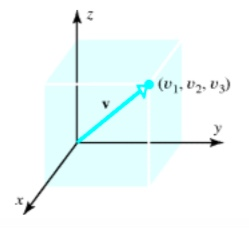
\includegraphics[scale=0.5]{figures_mvc/components}
\end{center}
The coordinate axes are labeled $x,y,$ and $z$, and are arranged such that if you take your right hand and curl your fingers from the positive $x$-axis toward the positive $y$-axis, your thumb points along the positive $z$-axis. Such a coordinate system is called \emph{right-handed}. Again, we find the set of all vectors in three dimensions is in 1-1 correspondence with the set $\R^3=\{(x,y,z) \mid x,y,z \in \R\}$. If $\varphi$ is the angle the vector makes with the positive $z$-axis and $\theta$ is the angle the projection of the vector onto the xy-plane, then the direction of a vector $\mathbf{x}$ is specified by the two angles $(\varphi,\theta)$. A little trigonometry shows that the correspondence is given by
\begin{align*}
	x&=||\mathbf{x}||\sin \varphi \cos \theta, \\
	y&=||\mathbf{x}||\sin \varphi \sin \theta, \\
	z&=||\mathbf{x}||\cos \varphi. \\
\end{align*}

\begin{exercise}
Work out these formulas from the diagram.	
\end{exercise}


The numbers $x,y,z$ are called the \emph{components} of the vector $\mathbf{x}$. We will denote the components of a given vector $\mathbf{v}$ by writing $\mathbf{v}=(v_1,v_2,v_3)$.

From the formula above for the components $x,y,z$, we see that the length of a vector $\mathbf{v}$ is given by an obvious generalization of the Pythagorean formula
\begin{equation}\label{eq:norm}
	||\mathbf{v}||=\sqrt{v_1^2+v_2^2+v_3^2}.
\end{equation}

\begin{exercise}
	Use the formulas for $x,y,z$ above to prove this.
\end{exercise}


\subsubsection{Vector arithmetic in coordinates}
We now derive the rule for vector addition in terms of components. Given vectors $\mathbf{v}$ and $\mathbf{w}$, we wish to find the components of $\mathbf{v}+\mathbf{w}$. According to the tip-to-tail rule, the $\mathbf{v}+\mathbf{w}$ is given by translating the vector $\mathbf{w}$ so that its initial point coincides with the terminal point of $\mathbf{v}$. This translation moves the $x$-coordinate of $\mathbf{w}$ by $v_1$ units in the $x$-direction, the $y$-coordinate by $v_2$ units in the $y$-direction, and the $z$-coordinate by $v_3$ units in the $z$-direction. That is, 
\begin{align*}
	(w_1,w_2,w_2) \mapsto (v_1+w_1,v_2+w_2,v_3+w_3)
\end{align*}
Thus, the coordinates of $\mathbf{v}+\mathbf{w}$ are given by
\begin{align*}
	\mathbf{v}+\mathbf{w}=(v_1+w_1,v_2+w_2,v_3+w_3).
\end{align*}
\begin{defn}[Vector addition in components]\label{def:vector_addition}
	In terms of components, the rule for vector addition is given by
	\begin{align*}
		(v_1,v_2,v_3)+(w_1,w_2,w_3)=(v_1+w_1,v_2+w_2,v_3+w_3).
	\end{align*}
\end{defn}

This formula is illustrated in the diagram on the left in Figure \ref{fig:vector_operations}.

\begin{example}
Let $\mathbf{v}=(1,2,3)$ and $\mathbf{w}=(-3,1,7)$. Then 
\begin{align*}
	\mathbf{v}+\mathbf{w}=(-2,3,10).
\end{align*}	
\end{example}


\begin{exercise}
	\begin{enumerate}[(a)]
		\item Use the formula in Definition \ref{def:vector_addition} to show that vector addition is commutative.
		\item Use the formula in Definition \ref{def:vector_addition} to show that vector addition is associative.
		\item What are the components of the zero vector?
		\item Given a vector $\mathbf{v}=(v_1,v_2,v_3)$, what are the components of $-\mathbf{v}$ (the additive inverse of $\mathbf{v}$)?
	\end{enumerate}
\end{exercise}

\begin{prop}\label{prop:scalar_multiple_formula}
If $\mathbf{v}=(v_1,v_2,v_3)$ is a vector and $k$ a scalar, then the components of the scalar multiple $k\mathbf{v}$ of $\mathbf{v}$ by $k$ are given by
\begin{align*}
	k\mathbf{v}=(kv_1,kv_2,kv_3)
\end{align*}	
\end{prop}

\begin{exercise}
	Use equation \eqref{eq:norm} to prove this.
\end{exercise}

\begin{example}
Let $\mathbf{v}=(1,2,3)$ and $k=3$. Then
\begin{align*}
	k\mathbf{v}=(3,6,9).
\end{align*}	
\end{example}

The formula in \eqref{prop:scalar_multiple_formula} is illustrated in the diagram on the right in Figure \ref{fig:vector_operations}.


\begin{exercise}
Use the formula in Proposition \eqref{prop:scalar_multiple_formula} to prove Theorem \eqref{thm:properties_of_scalar_multiplication}.	
\end{exercise}

\begin{exercise}
Use the formula in Proposition \eqref{prop:scalar_multiple_formula} to prove Corollary \eqref{cor:scalar_mult}.	
\end{exercise}

\begin{figure}\label{fig:vector_operations}
	\begin{center}
	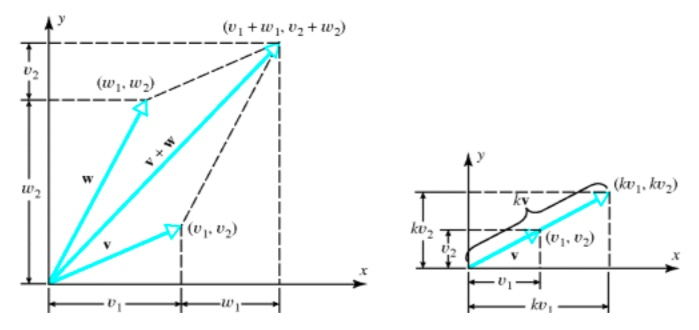
\includegraphics[scale=0.5]{figures_mvc/vector_operations}
\end{center}	
\caption{Vector operations in components.}
\end{figure}

\begin{exercise}
Prove that if $\mathbf{v}=(v_1,v_2,v_3)$ and $\mathbf{w}=(w_1,w_2,w_3)$, then
\begin{align*}
	\mathbf{v}-\mathbf{w}=(v_1-w_1,v_2-w_2,v_3-w_3).
\end{align*}	
\end{exercise}

From \ref{def:vector_subtraction}, we see that the vector $\mathbf{v}-\mathbf{w}$ originates from the point $(w_1,w_2,w_3)$ and terminates at the point $(v_1,v_2,v_3)$. \fixme{Insert graphic.} The distance between these two points is therefore given by
\begin{align*}
	||\mathbf{v}-\mathbf{w}||=\sqrt{(v_1-w_1)^2+(v_2-w_2)^2+(v_3-w_3)^2}.
\end{align*}

\begin{exercise}
\begin{enumerate}[(a)]
	\item Find the components of the vector $\overrightarrow{P_1P_2}$ with initial point $P_1(2,-1,4)$ and terminal point $P_2(7,5,-8)$.
	\item Find the distance between $P_1(2,-1,4)$ and $P_2(7,5,-8)$.
\end{enumerate}	
\end{exercise}

{\color{red} \flushleft {\bf Solution:} 
\begin{enumerate}[(a)]
	\item The components of $\overrightarrow{P_1P_2}$ are given by
	\begin{align*}
		\overrightarrow{P_1P_2}=(7-2,5-(-1),-8-4)=(5,6,-12)
	\end{align*}
	\item The distance between $P_1$ and $P_2$ is 
	\begin{align*}
		||\overrightarrow{P_1P_2}||=\sqrt{5^2+6^2+(-12)^2}=\sqrt{205}.
	\end{align*}
\end{enumerate}}

\subsubsection{Unit vectors}
\begin{defn}[Unit vector]
	A \emph{unit vector} is a vector of unit length. That is, a vector ${\bf v}$ such that $||{\bf v}||=1$.
\end{defn}

\begin{prop}[Normalizing a vector]
	If ${\bf v}\neq 0$, then ${\bf v}/||{\bf v}||$ is a unit vector in the direction of ${\bf v}$. The unit vector ${\bf v}/||{\bf v}||$ is often denoted ${\bf \hat{v}}$ and the process of forming ${\bf \hat{v}}$ from ${\bf v}$ is called \ti{normalizing} ${\bf v}$.
\end{prop}

\begin{pf}
Since ${\bf v}\neq 0$, $||{\bf v}|| \neq 0$, so we can multiply ${\bf v}$ by $1/||{\bf v}||$. Computing the length of $||\frac{{\bf v}}{||{\bf v}||}||$, we see that 
\begin{align*}
	||\frac{{\bf v}}{||{\bf v}||}||&=\frac{||{\bf v}||}{||{\bf v}||}=1,
\end{align*} 
hence ${\bf v}/||{\bf v}||$ is a unit vector. Since ${\bf v}/||{\bf v}||$ is a scalar multiple of ${\bf v}$ (by $k=1/||{\bf v}||$) it is parallel to ${\bf v}$, and since $k>0$, ${\bf v}/||{\bf v}||$ has the same orientation as $\mathbf{v}$.
\end{pf}

\begin{example}
	We can express any nonzero vector ${\bf v}$ as a product of its magnitude and direction by means of the formula \footnote{Note that this is a generalization of the formula $x=|x|\frac{x}{|x|}$ for a nonzero real number $x$.}
	\begin{align*}
		{\bf v}=||{\bf v}||\frac{{\bf v}}{||{\bf v}||}.
	\end{align*}
	For example, taking ${\bf v}=(1,-2,3)$,
	\begin{align*}
		||{\bf v}||=\sqrt{1^2+(-2)^2+3^2}=\sqrt{14}
	\end{align*}
	and thus
	\begin{align*}
		{\bf v}=\sqrt{14}(\frac{1}{\sqrt{14}},\frac{-2}{\sqrt{14}},\frac{3}{\sqrt{14}}).
	\end{align*}
\end{example}


\begin{defn}[Standard unit vectors]
	 The \ti{standard unit vectors} for $\mathbb{R}^3$ are the vectors
	\begin{align*}
		{\bf i}&=(1,0,0), \\
		{\bf j}&=(0,1,0), \\
		{\bf k}&=(0,0,1). \\
	\end{align*}
These vectors are unit vectors pointing along the $x$-, $y$-, and $z$-axes, respectively. \footnote{The standard unit vectors $({\bf i},{\bf j},{\bf k})$ are also commonly denoted as $({\bf e}_1, {\bf e}_2, {\bf e}_3)$ or $({\bf \hat{x}}, {\bf \hat{y}}, {\bf \hat{z}})$.}	
\end{defn}
Using the standard unit vectors, we may write the vector ${\bf v}=(v_1,v_2,v_3)$ as $${\bf v}=v_1{\bf i}+v_2{\bf j}+v_3{\bf k}.$$
A sum of this form is said to be a \emph{linear combination} of the vectors ${\bf i},{\bf j},{\bf k}$. You should be comfortable working with both expressions for a vector $\mathbf{v}$ in terms of its components.

\begin{exercise}
Find a unit vector in the direction of the vector from $P_1(1,0,1)$ to $P_2(3,2,0)$.
\end{exercise}

{\color{red} \flushleft {\bf Solution:}
We find $\overrightarrow{P_1P_2}$ and normalize:
\begin{align*}
	\overrightarrow{P_1P_2}&=(3-1,2-0,0-1)=(2,2,-1), \\
	||\overrightarrow{P_1P_2}||&=\sqrt{2^2+2^2+(-1)^2}=3, \\
\end{align*}
and therefore the desired unit vector is given by
\begin{align*}
	\frac{\overrightarrow{P_1P_2}}{||\overrightarrow{P_1P_2}||}=(\frac{2}{3},\frac{2}{3},-\frac{1}{3}).
\end{align*}}

\begin{exercise}
Find a vector 6 units long in the direction of ${\bf v}=(2,2,-1)$.	
\end{exercise}

{\color{red} \flushleft {\bf Solution:}
The vector we want is 
\begin{align*}
6\frac{{\bf v}}{||{\bf v}||}=6\frac{(2,2,-1)}{\sqrt{2^2+2^2+(-1^2)}}=6\frac{(2,2,-1)}{3}=(4,4,-2).	
\end{align*}
}

\subsubsection{The dot product}
Two nonzero vectors ${\bf u}$ and ${\bf v}$ positioned so that their initial points coincide determine an angle $\theta \in [0,\pi]$, which is the angle between the two vectors.
\begin{center}
	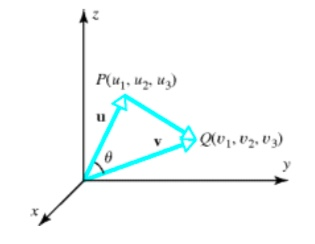
\includegraphics[scale=0.5]{figures_mvc/angle_uv}
\end{center}
Note that the information about $\theta$ is encoded in ${\bf u}-{\bf v}$, since if we fix the magnitudes of ${\bf u}$ and ${\bf v}$ and open the angle, then ${\bf u}-{\bf v}$ will also change. The fundamental relation satisfied by ${\bf u}, {\bf v}$ and $\theta$ is the law of cosines, which says that if ${\bf w}={\bf u}-{\bf v}$, then
\begin{equation}\label{eq:law_of_cosines}
	||{\bf w}||^2=||{\bf u}||^2+||{\bf v}||^2-2||{\bf u}|| \ ||{\bf v}||\cos \theta. 
\end{equation}
Let us make the following definition.
\begin{defn}[Dot product]
	The \ti{dot product} of two nonzero vectors ${\bf u}$ and ${\bf v}$ is defined by
	\begin{equation}\label{eq:dot_product_def}
		{\bf u}\cdot {\bf v}=||{\bf u}|| \ ||{\bf v}||\cos\theta.
	\end{equation} 
\end{defn}
The angle between two vectors ${\bf u}$ and ${\bf v}$ is then given by
\begin{equation}\label{eq:angle_uv}
	\theta=\cos^{-1}\left(\frac{{\bf u}\cdot {\bf v}}{||{\bf u}|| \ ||{\bf v}||}\right),
\end{equation}	
and we see that
\begin{itemize}
	\item $\theta$ is acute if ${\bf u} \cdot {\bf v} > 0$.
	\item $\theta$ is obtuse if ${\bf u} \cdot {\bf v} < 0$.
	\item $\theta$ is right if ${\bf u} \cdot {\bf v} = 0$.
\end{itemize}

Since the dot product takes as input two vectors and returns a scalar, it is also called the \ti{scalar product}. Note that from Eq. \eqref{eq:law_of_cosines}, we can write ${\bf u}\cdot {\bf v}$ in terms of magnitudes only, as 
\begin{equation}\label{eq:dot_product_magnitudes}
	{\bf u}\cdot {\bf v}=\frac{||{\bf u}||^2+||{\bf v}||^2-||{\bf u}-{\bf v}||^2}{2}.
\end{equation}
Note that since this equation involves only lengths of segments and angles between segments, it holds in \emph{all} coordinate systems. However, it takes a particularly simple form in Cartesian coordinates. Writing out the norm of each vector in terms of its components gives

\begin{align*}
	{\bf u}\cdot {\bf v}&=\frac{u_1^2+u_2^2+u_3^2+v_1^2+v_2^2+v_3^2-(u_1-v_1)^2-(u_2-v_2)^2-(u_3-v_3)^2}{2}
\end{align*}
Expanding the binomials and cancelling like terms, we find
\begin{equation}
	{\bf u}\cdot {\bf v}=u_1v_1+u_2v_2+u_3v_2.
\end{equation}

\begin{exercise}
Compute the angle between the vectors ${\bf u}=(0,0,3)$ and ${\bf v}=(\sqrt{2},0,\sqrt{2})$.	
\end{exercise}

{\color{red} \flushleft {\bf Solution:} The angle between these vectors is
\begin{align*}
	\theta=\cos^{-1}\left(\frac{0(\sqrt{2}+0(0)+3(\sqrt{2}))}{3(2)}\right)=\cos^{-1}\left(\frac{1}{\sqrt{2}}\right)=\frac{\pi}{4}.
\end{align*}}

\begin{exercise}
	Find the angle between a diagonal of a cube and one of its edges.
\end{exercise}

{\color{red} \flushleft {\bf Solution:}
Let $s$ be the length of an edge and place the cube in the first octant so that one vertex is at the origin and two edges are along the $x$- and $y$-axes.
\begin{center}
	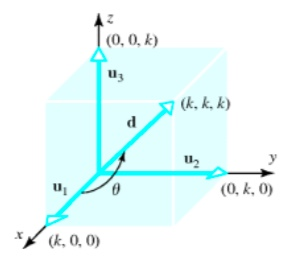
\includegraphics[scale=0.5]{figures_mvc/cube_coordinates}
\end{center}
If we let ${\bf u}_1=(s,0,0), {\bf u}_1=(0,s,0)$, and ${\bf u}_3=(0,0,s)$, then the vector
\begin{align*}
	{\bf d}=(s,s,s)={\bf u}_1+{\bf u}_2+{\bf u}_3
\end{align*}
is a diagonal of the cube. The angle between ${\bf d}$ and ${\bf u}_1$ is 
\begin{align*}
	\theta &=\cos^{-1}\left(\frac{{\bf u}_1 \cdot {\bf d}}{||{\bf u}_1 || \ || {\bf d}||}\right) \\
	&=\cos^{-1}\left(\frac{s^2}{(s)(\sqrt{3s^2})}\right)  \\
	&=\cos^{-1}\left(\frac{1}{\sqrt{3}}\right) \\
	&\approx 54.74^\circ.
\end{align*}
}

\begin{prop}[Properties of the dot product]
	Let ${\bf a}, {\bf b}, {\bf c}, {\bf d}$ be vectors and $k$ any scalar. Then 
	\begin{enumerate}[(1)]
		\item ${\bf a}\cdot {\bf b}={\bf b} \cdot {\bf a}$
		\item $(k {\bf a})\cdot {\bf b}={\bf a}\cdot (k{\bf b})=k({\bf a}\cdot {\bf b})$
		\item ${\bf a}\cdot ({\bf b}+{\bf c})={\bf a}\cdot {\bf b}+{\bf a}\cdot {\bf c}$
		\item $({\bf a}+{\bf b})\cdot {\bf a}={\bf a}\cdot {\bf c}+{\bf b}\cdot {\bf c}$
		\item $({\bf a}+{\bf b})\cdot ({\bf c}+{\bf d})={\bf a}\cdot {\bf c}+{\bf a}\cdot {\bf d}+{\bf b}\cdot {\bf c}+{\bf b}\cdot {\bf d}$
		\item ${\bf a} \cdot {\bf a}=||{\bf a}||^2$
	\end{enumerate}
\end{prop}

\begin{pf}
Each of these can be proved by writing out the vectors in components. For example, to prove (1)
\begin{align*}
	{\bf a}\cdot {\bf b}&=a_1b_1+a_2b_2+a_3b_3 \\
	&=b_1a_1+b_2a_2+b_3a_3 \\
	&={\bf b}\cdot {\bf a}
\end{align*}
Properties (2)-(6) are proved similarly. Note that (5) follows from (3) and (4), but is included for emphasis since it is used frequently. 	
\end{pf}

\fixme{Add exercises using these properties.}

Note, however, the differences between the dot product and ordinary multiplication. For instance, one might ask, ``Is the dot product associative?". This question doesn't even make any sense for the dot product, as expressions such as ${\bf a}\cdot ({\bf b}\cdot {\bf c})$ are not defined, since ${\bf a}$ is a vector and $({\bf b}\cdot {\bf c})$ is a scalar, and one can only form the dot product between two vectors. 

\subsubsection{Orthogonal vectors}
While writing vectors in component form has the advantage of facilitating many computations, this form seems to obscure geometric relations between vectors.
For instance, the two vectors
\begin{align*}
	{\bf u}&=(3,-2,1) \\
	{\bf v}&=(0,2,4).
\end{align*}
are orthogonal (perpendicular), but this does not seem obvious in the given form. We know from right triangle trigonometry that right angles are very special, so it would be nice to have a way to check if two vectors written in component form are perpendicular. Fortunately, the dot product gives us an easy way to determine this. 
\begin{prop}[Orthogonal vectors]\label{prop:orthogonal_vectors}
	Two nonzero vectors ${\bf a}$ and ${\bf b}$ are orthogonal if and only if ${\bf a}\cdot {\bf b}=0$.
\end{prop}

\begin{pf}
	The dot product of ${\bf a}$ and ${\bf b}$ is given by
\begin{align*}
	{\bf a}\cdot {\bf b}=||{\bf a}|| \ ||{\bf b}||\cos \theta.
\end{align*}	
If ${\bf a}$ and ${\bf b}$ are non-zero, then $||{\bf a}||$ and $||{\bf b}||$ are greater than zero, so ${\bf a}\cdot {\bf b}=0$ if and only if $\theta=\frac{\pi}{2}$, that is, if and only if ${\bf a}$ and ${\bf b}$ are orthogonal. 
\end{pf}

What if ${\bf b}={\bf 0}$? In this case, $\theta$ is not well-defined, since we have defined ${\bf 0}$ to be any vector with zero magnitude, independently of direction. For Proposition \ref{prop:orthogonal_vectors} to hold even if ${\bf a}$ or ${\bf b}$ are ${\bf 0}$, we simply define ${\bf a}\cdot {\bf b}=0$ if one of the vectors is the zero vector. With this definition, the zero vector is orthogonal to every vector, including itself.

\begin{example}
The two vectors in the example above	
\begin{align*}
	{\bf u}&=(3,-2,1) \\
	{\bf v}&=(0,2,4).
\end{align*}
are orthogonal since ${\bf u}\cdot {\bf v}=3(0)-2(2)+1(4)=-4+4=0$.
\end{example}

\begin{example}
	The standard unit vectors for $\mathbb{R}^3$ are mutually orthogonal. One can easily verify that 
	\begin{align*}
		{\bf e}_i \cdot {\bf e_j}=\delta_{ij}
	\end{align*}
where 
\begin{align*}
	\delta_{ij} \equiv \begin{cases}
		1 \text{ if } i=j, \\
		0 \text{ if } i \neq j
	\end{cases}
\end{align*}
is called the \ti{Kronecker delta symbol}.
\end{example}

These examples illustrate another difference between the dot product of two vectors and the ordinary product of two numbers. For two real numbers, if $ab=0$, then either $a=0$ or $b=0$. These examples clearly show that if ${\bf a}\cdot {\bf b}=0$, then it need not be true that either ${\bf a}=0$ or ${\bf b}=0$.
\subsubsection{Projection of a vector}
Let ${\bf a}$ be a nonzero vector, ${\bf \hat{a}}=\frac{{\bf a}}{||{\bf a}||}$ the unit vector obtained by normalizing ${\bf a}$, and ${\bf b}$ another vector. Then Eq. \eqref{eq:dot_2} shows that
\begin{align*}
	{\bf \hat{a}}\cdot {\bf b}=\frac{{\bf a}}{||{\bf a}||} \cdot {\bf b}=||{\bf b}||\cos \theta
\end{align*} 
is the component of ${\bf b}$ in the direction of ${\bf a}$. Multiplying by ${\bf \hat{a}}$, we get a vector parallel to ${\bf a}$ whose magnitude is the component of ${\bf b}$ along ${\bf a}$.

\begin{defn}[Vector projection]
	The vector $\text{proj}_{\bf a}{\bf b}\equiv ({\bf \hat{a}}\cdot {\bf b}){\bf \hat{a}}=||{\bf b}||\cos \theta {\bf \hat{a}}$ is called the \ti{projection of ${\bf b}$ onto ${\bf a}$}.
\end{defn}
Geometrically, the projection of ${\bf b}=\overrightarrow{PQ}$ onto ${\bf a}=\overrightarrow{PS}$ is the vector $\overrightarrow{PR}$ determined by dropping a perpendicular from $Q$ to the line $PS$. \footnote{Note that by using the definitions of the dot product and the norm of ${\bf a}$, one may produce many equivalent expressions for $\text{proj}_{\bf a}{\bf b}$:
\begin{align*}
	\text{proj}_{\bf a}{\bf b}&=(||{\bf b}||\cos \theta){\bf \hat{a}} \\
	&=({\bf \hat{a}}\cdot {\bf b}){\bf \hat{a}} \\
	&=\left(\frac{{\bf a}\cdot {\bf b}}{||{\bf a}||}\right)\frac{{\bf a}}{||{\bf a}||} \\
	&=\left(\frac{{\bf b}\cdot {\bf a}}{{\bf a}\cdot {\bf a}}\right){\bf a}
\end{align*}
The first of these is perhaps the easiest to remember, as it makes most transparent the relation to elementary right triangle trigonometry.}

\begin{center}
	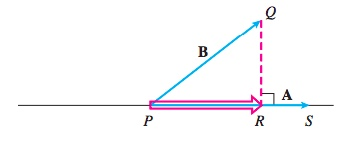
\includegraphics[scale=0.5]{figures_mvc/vector_projection_def}
\end{center}
Physically, if ${\bf b}$ represents a force, then $\text{proj}_{\bf a}{\bf b}$ is the effective force in the ${\bf a}$ direction.

\begin{center}
	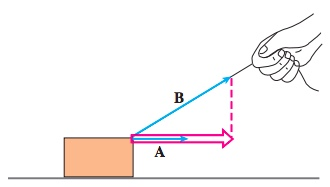
\includegraphics[scale=0.5]{figures_mvc/effective_force_box}
\end{center}	

It is often desirable to express a vector ${\bf b}$ as a sum of two orthogonal vectors. For instance, in mechanics we frequently decompose forces in this way so that we may treat a two-dimensional problem as two one-dimensional problems. We can easily express a vector ${\bf b}$ as such a sum of two vectors, one parallel to some nonzero vector ${\bf a}$ and one orthogonal to ${\bf a}$, in terms of the projection of ${\bf b}$ along ${\bf a}$:
\begin{equation}
\begin{split}
	{\bf b}&={\bf b}_{\parallel}+{\bf b}_{\perp} \\
	&=\text{proj}_{\bf a}{\bf b}+({\bf b}-\text{proj}_{\bf a}{\bf b}).
\end{split}
\end{equation}

\begin{center}
	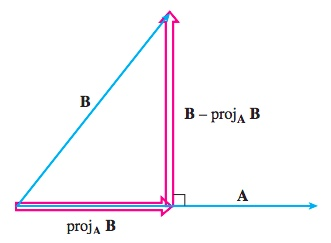
\includegraphics[scale=0.5]{figures_mvc/sum_of_orthogonal_vectors}
\end{center}

\begin{exercise}
	Express ${\bf b}=2{\bf e}_1+{\bf e}_2-3{\bf e}_3$ as the sum of a vector parallel to ${\bf a}=3{\bf e}_1-{\bf e}_2$ and a vector orthogonal to ${\bf a}$.
\end{exercise}

{\color{red} \flushleft {\bf Solution:}
Since ${\bf \hat{a}}\equiv \frac{{\bf a}}{||{\bf a}||}=\frac{3{\bf e}_1-{\bf e}_2}{\sqrt{10}}$, we can write ${\bf b}={\bf b}_{\parallel}+{\bf b}_{\perp}$ with  
\begin{align*}
	{\bf b}_{\parallel}&=({\bf \hat{a}}\cdot {\bf b}){\bf {\hat{a}}}=\frac{1}{2}(3{\bf e}_1-{\bf e}_2)=\frac{1}{2}{\bf a} \\
	{\bf b}_{\perp}&={\bf b}-{\bf b}_{\parallel}=\frac{1}{2}{\bf e}_1+\frac{3}{2}{\bf e}_2-3{\bf e}_3.
\end{align*}}

\subsection{Equations of lines and planes}
\subsubsection{Lines in space}
The coordinate systems of analytic geometry allow us to consider geometric objects such as lines and planes in terms of vectors. These geometric ideas will give us valuable intuition later on in the course when we take a more abstract point of view toward vectors.

First let us recall that any two points define a line. Equivalently, we can also determine a line if we know one point on the line and the slope of the line. 

Let us now work in Cartesian coordinates. Suppose $L$ is a line passing through a point $P_0(x_0,y_0,z_0)$ and parallel to a vector ${\bf v}=v_1{\bf e}_1+v_2{\bf e}_2+v_3{\bf e}_3$. Now let $P(x,y,z)$ be any point in space. In which case will $P(x,y,z)$ to be on the line? This will be the case if the vector $\overrightarrow{P_0P}$ is parallel to ${\bf v}$, that is, if $\overrightarrow{P_0P}$ is a scalar multiple of ${\bf v}$. Therefore,
\begin{defn}[Vector equation for a line]
	The line through $P_0(x_0,y_0,z_0)$ and parallel of ${\bf v}$ is the set of all points $P(x,y,z)$ such that $\overrightarrow{P_0P}=t{\bf v}$, with $-\infty < t < \infty$. This equation is called the \ti{vector equation} of the line.
\end{defn}
In terms of Cartesian coordinates, the vector equation for the line becomes
\begin{align*}
	(x-x_0){\bf e}_1+(y-y_0){\bf e}_2+(z-z_0){\bf e}_3&=t(v_1{\bf e}_1+v_2{\bf e}_2+v_3{\bf e}_3) \\
	&=tv_1{\bf e}_1+tv_2{\bf e}_2+tv_3{\bf e}_3
\end{align*}
which implies
\begin{align*}
	(x-x_0-tv_1){\bf e}_1+(y-y_0-tv_2){\bf e}_2+(z-z_0-tv_3){\bf e}_3={\bf 0}
\end{align*}
and hence
\begin{equation}\label{eq:parametric_equations_line}
	x=x_0+tv_1, \hspace{0.25cm} y=y_0+tv_2, \hspace{0.25cm} z=z_0+tv_3.
\end{equation}
Thus, the vector equation of the line is equivalent to the three scalar equations in Eq. \eqref{eq:parametric_equations_line}, each of which is the usual equation for a line with slope $v_i$ in one variable $t$.

\begin{defn}[Parametric equations for a line]
	The standard parametrization of the line through $P_0(x_0,y_0,z_0)$ and parallel to ${\bf v}=v_1{\bf e}_1+v_2{\bf e}_2+v_3{\bf e}_3$ is given by
	\begin{align*}
		x=x_0+tv_1, \hspace{0.25cm} y=y_0+tv_2, \hspace{0.25cm} z=z_0+tv_3.
	\end{align*}
	These equations are called the (standard) \ti{parametric equations} for the line.
\end{defn}

\begin{exercise}
Find the parametric equations for the line through $(-2,0,4)$ and parallel to ${\bf v}=2{\bf e}_1+4{\bf e}_2-2{\bf e}_3$.	
\end{exercise}

{\color{red} \flushleft {\bf Solution:}
Plugging into Eq. \eqref{eq:parametric_equations_line} gives
\begin{align*}
	x=-2+2t, \hspace{0.25cm} y=4t, \hspace{0.25cm} z=4-2t.
\end{align*}}
\begin{center}
	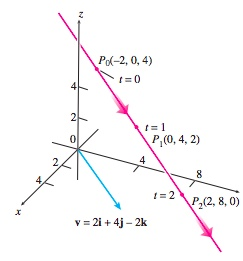
\includegraphics[scale=0.5]{figures_mvc/parametrized_line_example_1}
\end{center}

\begin{example}
	Find parametric equations for the line through $P(-3,2,-3)$ and $Q(1,-1,4)$.
\end{example}

{\color{red} \flushleft {\bf Solution:}
The vector from $P$ to $Q$ is 
\begin{align*}
	\overrightarrow{PQ}&=(1-(-3), -1-2, 4-(-3)) \\
	&=(4,-3,7).
\end{align*}
We take this vector to be our ``${\bf v}$". The point $P_0$ could be either $P$ or $Q$. Arbitrarily choosing it to be $Q$, Eq. \eqref{eq:parametric_equations_line} gives
\begin{align*}
	x=1+4t, \hspace{0.25cm} y=-1-3t, \hspace{0.25cm} z=4+7t.
\end{align*}}

\begin{exercise}
Parametrize the line segment joining the points $P(-3,2,-3)$ and $Q(1,-1,4)$.	
\end{exercise}
{\color{red} \flushleft {\bf Solution:}
We have seen in the previous exercise that the  parametric equations 
\begin{align*}
	x=1+4t, \hspace{0.25cm} y=-1-3t, \hspace{0.25cm} z=4+7t.
\end{align*}
describe an infinite line containing $P$ and $Q$ when we take $-\infty < t < \infty$. To describe the line segment joining $P$ and $Q$, we simply restrict the domain of $t$. We see that the line passes through $P$ at $t=-1$ and $Q=0$. So the line segment joining $P$ and $Q$ is given by 

\begin{align*}
	x=1+4t, \hspace{0.25cm} y=-1-3t, \hspace{0.25cm} z=4+7t.
\end{align*}

with $-1 < t < 0$.}

\subsubsection{Planes in space}
Whereas a line is determined by any two points, a plane is determined by any \ti{three} non-collinear points. Similar to a line, which was equivalently determined by a single point and a slope, a plane can also be determined by a single point and a ``slope". The direction of the plane is determined by a normal vector ${\bf n}=n_1{\bf e}_1+n_2{\bf e}_2+n_3{\bf e}_3$. 

Let us now repeat the question we asked before: given a point $P_0(x_0,y_0,z_0)$ on the plane and a vector ${\bf n}$ normal to the plane, what is the condition for an arbitrary point in space $P(x,y,z)$ to lie on the plane? If $P$ lies in the plane, the $\overrightarrow{P_0P}$ is a vector lying in the plane. Then, since ${\bf n}$ is normal to the plane, we must have that ${\bf n} \cdot \overrightarrow{P_0P}=0$.

\begin{center}
	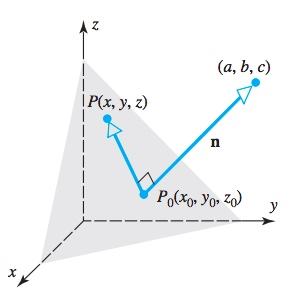
\includegraphics[scale=0.5]{figures_mvc/vector_equation_of_a_plane}
\end{center}

\begin{defn}[Vector equation for a plane]
	The \ti{vector equation} of the plane through $P_0(x_0,y_0,z_0)$ and normal to ${\bf n}=n_1{\bf e}_1+n_2{\bf e}_2+n_3{\bf e}_3$ is given by
	\begin{equation}
		{\bf n} \cdot \overrightarrow{P_0P}=0.
	\end{equation}
\end{defn}

As before, we can expand this equation in Cartesian coordinates to obtain

\begin{defn}[The component equation of a plane]
	The component equation of a plane through $P_0(x_0,y_0,z_0)$ and normal to ${\bf n}=n_1{\bf e}_1+n_2{\bf e}_2+n_3{\bf e}_3$ is given by
	\begin{equation}
		n_1(x-x_0)+n_2(y-y_0)+n_3(z-z_0)=0.
	\end{equation}
	This can be simplified to 
	\begin{equation}
		n_1x+n_2y+n_3z=c
	\end{equation}
	where $c=n_1x_0+n_2y_0+n_3z_0$.
\end{defn}

\begin{exercise}
Find an equation for the plane through $P_0(-3,0,7)$ perpendicular to ${\bf n}=(5,2,-1)$.	
\end{exercise}

{\color{red} \flushleft {\bf Solution:}
The component equation is 
\begin{align*}
	5(x-(-3))+2(y-0)+(-1)(z-7)=0,
\end{align*}
Simplifying, we obtain
\begin{align*}
	5x+15+2y-z+7&=0 \\
	5x+2y-z&=-22.
\end{align*}}

\begin{exercise}
Find the point where the line 
\begin{align*}
	x=\frac{8}{3}+2t, \hspace{0.25cm} y=2t, \hspace{0.25cm} z=1+t
\end{align*}	
intersects the plane $3x+2y+6z=6$.
\end{exercise}

{\color{red} \flushleft {\bf Solution:}
The point $(\frac{8}{3}+2t, 2t, 1+t)$ lies in the plane if its coordinates satisfy the equation of the plane; that is, if
\begin{align*}
	3(\frac{8}{3}+2t)+2(-2t)+6(1+t)=6
\end{align*}
This has a solution at $t=-1$, so the point of intersection is 
\begin{align*}
	(x,y,z)\vert_{t=-1}=(\frac{2}{3},2,0).
\end{align*}}

\begin{exercise}
\begin{enumerate}[(a)]
	\item Find a vector parallel to the line of intersection of the planes $3x-6y-2z=15$ and $2x+y-2z=5$.	
	\item Find parametric equations for the line in which these planes intersect.
\end{enumerate}
\end{exercise}

\end{document}

